\subsection{Overview of Artificial Intelligence-based Approaches}

Artificial intelligence is often used in different contexts; therefore, it is necessary to define what is meant by AI-based approaches and which different approaches exist. It is a leading technology in the current digital transformation and is crucial for advancing the fourth industrial revolution \cite{AI-Definition}.\\
The goal of AI is to create machines that can perform tasks that typically require human intelligence, such as understanding natural language and recognizing patterns in data. In particular, the detection of patterns is of relevance in this work. The different AI-based approaches can be divided into two subcategories \cite{AI-Definition}:
\begin{figure}[H]
  \centering
  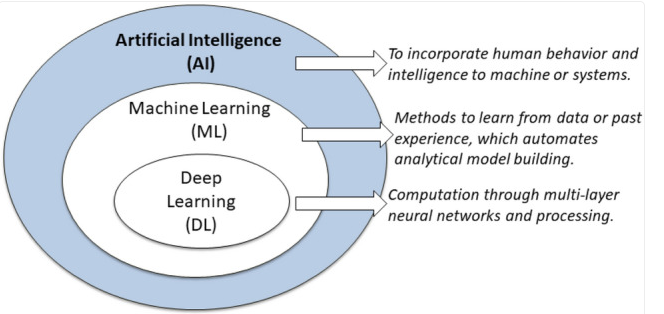
\includegraphics[width=0.7\textwidth]{pics/AI_approaches.png}
  \caption{An illustration of the position of Machine Learning and Deep Learning within the area of Artificial Intelligence \cite{AI-Definition}}
  \label{fig:AI_approaches}
\end{figure}
These can be further divided into three categories:
\begin{itemize}
  \item \textbf{Supervised Learning:} This approach involves learning from labeled data to identify patterns and make predictions. It is commonly used in tasks such as email spam classification or price prediction, where the algorithm is trained on known input-output pairs.
  \item \textbf{Unsupervised Learning:} This data-driven method is used to uncover hidden patterns in unlabeled data. Techniques such as clustering and dimensionality reduction are applied to identify structures within the data, for example, to segment customer groups or discover business models.
  \item \textbf{Semi-Supervised Learning:} This approach combines aspects of both supervised and unsupervised learning by utilizing a small amount of labeled data alongside a larger pool of unlabeled data. It is particularly useful when labeling data is expensive or time-consuming, but large amounts of unlabeled data are available.\\
\cite{AI-Definition}\\
\end{itemize}

In the following table, the different approaches are categorized alongside their corresponding machine learning architectures. This allows identification of the advantages and disadvantages of each method and provides a clearer understanding of which approach is most suitable for producing actionable results in real-world deployments.
\begin{table}[H]
	\centering
	\begin{tabular}{|l|p{3.5cm}|p{4cm}|p{4cm}|}
		\hline
		\textbf{Approach} & \textbf{Examples} & \textbf{Advantages} & \textbf{Disadvantages}\\
		\hline
		Supervised Learning & Decision Trees, \newline Random-Forest, \newline LSTM & High prediction accuracy, \newline Clear objectives & Requires a lot of labeled data, \newline Risk of overfitting\\
		\hline
		Unsupervised Learning & K-Means, \newline Isolation-Forest & Finds patterns without labels, \newline Useful for unlabeled data & Hard to interpret, \newline No clear target\\
		\hline
		Semi-Supervised Learning & Self-training & Improves performance with few labeled data points & Complex to implement\\
		\hline
	\end{tabular}
	\caption{Comparison of machine learning approaches with examples, advantages, and disadvantages \cite{AI-Definition}.}
    \label{tab:AI_approaches}
\end{table}

After providing an overview of the different machine learning approaches, the following chapter delves deeper into the field by examining various methods for anomaly detection and identifying the most effective models for detecting typical anomalies.
